\documentclass[a4paper, 12pt]{extarticle}
\usepackage[dvipsnames]{xcolor}
\usepackage[top=70pt,bottom=70pt,left=48pt,right=46pt]{geometry}
\definecolor{header}{RGB}{252, 171, 16}
\definecolor{defenition}{RGB}{248, 51, 60}
\definecolor{main_title}{RGB}{43, 158, 179}
\definecolor{sub_header}{RGB}{68, 175, 105}
\usepackage[english, russian]{babel}
\usepackage[utf8]{inputenc}
\usepackage{amsmath}
\usepackage[most]{tcolorbox}
\usepackage{listings}
\usepackage{graphicx}
\usepackage{amsmath}
\usepackage{lettrine}
\title{\textcolor{main_title}{Оптика лазерных пучков}}

\author{
    Нечаева Дарья - ФФКЭ гр. Б04-103 \and
    Ульянова Мария - ФФКЭ гр. Б04-103 \and
    Шмаков Владимир - ФФКЭ гр. Б04-103 
}


\newtcolorbox{fequation}[1][]{ams equation*,size=small,#1}








\begin{document}
\maketitle



\section*{\textcolor{header}{Цель работы}}
    Определить координату перетяжки для излучения от двух лазеров.



\section*{\textcolor{header}{Методика}}

\subsection*{\textcolor{sub_header}{Оборудование}}
\begin{itemize}
    \item Полупроводниковый лазер
    \item Гелий - неоновый лазер
    \item Линза
    \item Фотодиод
    \item Вольтметр
    \item Микрометрический винт
\end{itemize}

\subsection*{\textcolor{sub_header}{Экспериментальная установка}}
\begin{figure}[htbp]
    \centering
    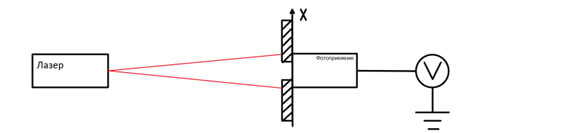
\includegraphics[width = 0.8\textwidth]{ustanovka.jpg}
    \caption{Схема экспериментальной установки}
    \label{<label>}
\end{figure}
Экспериментальная установка представляет собой лазер, направленный на фотоприемник с щелью, расположенные на подложке, которая перемещается с помощью микрометрического винта. Тем самым, перемещая щель вдоль оси X, мы можем изучить поперечную структуру лазерного пучка и определить координату перетяжки.
\section*{\textcolor{header}{Обработка экспериментальных данных}}

Снимем зависимость ширины пучка от расстояния между фотодиодом и He-Ne лазером. Будем находить максимум интенсивности на определенной координате. Ширину будем определять по уменьшению интенсивности в $1/e^2$, сдвигая подложку с помощью микрометрического винта. 
Приближая зависимость параболой, можно определить координату перетяжки:
$x \sim 50.4$ см (смотрите рисунок 2).
\begin{figure}[htbp]
    \centering
    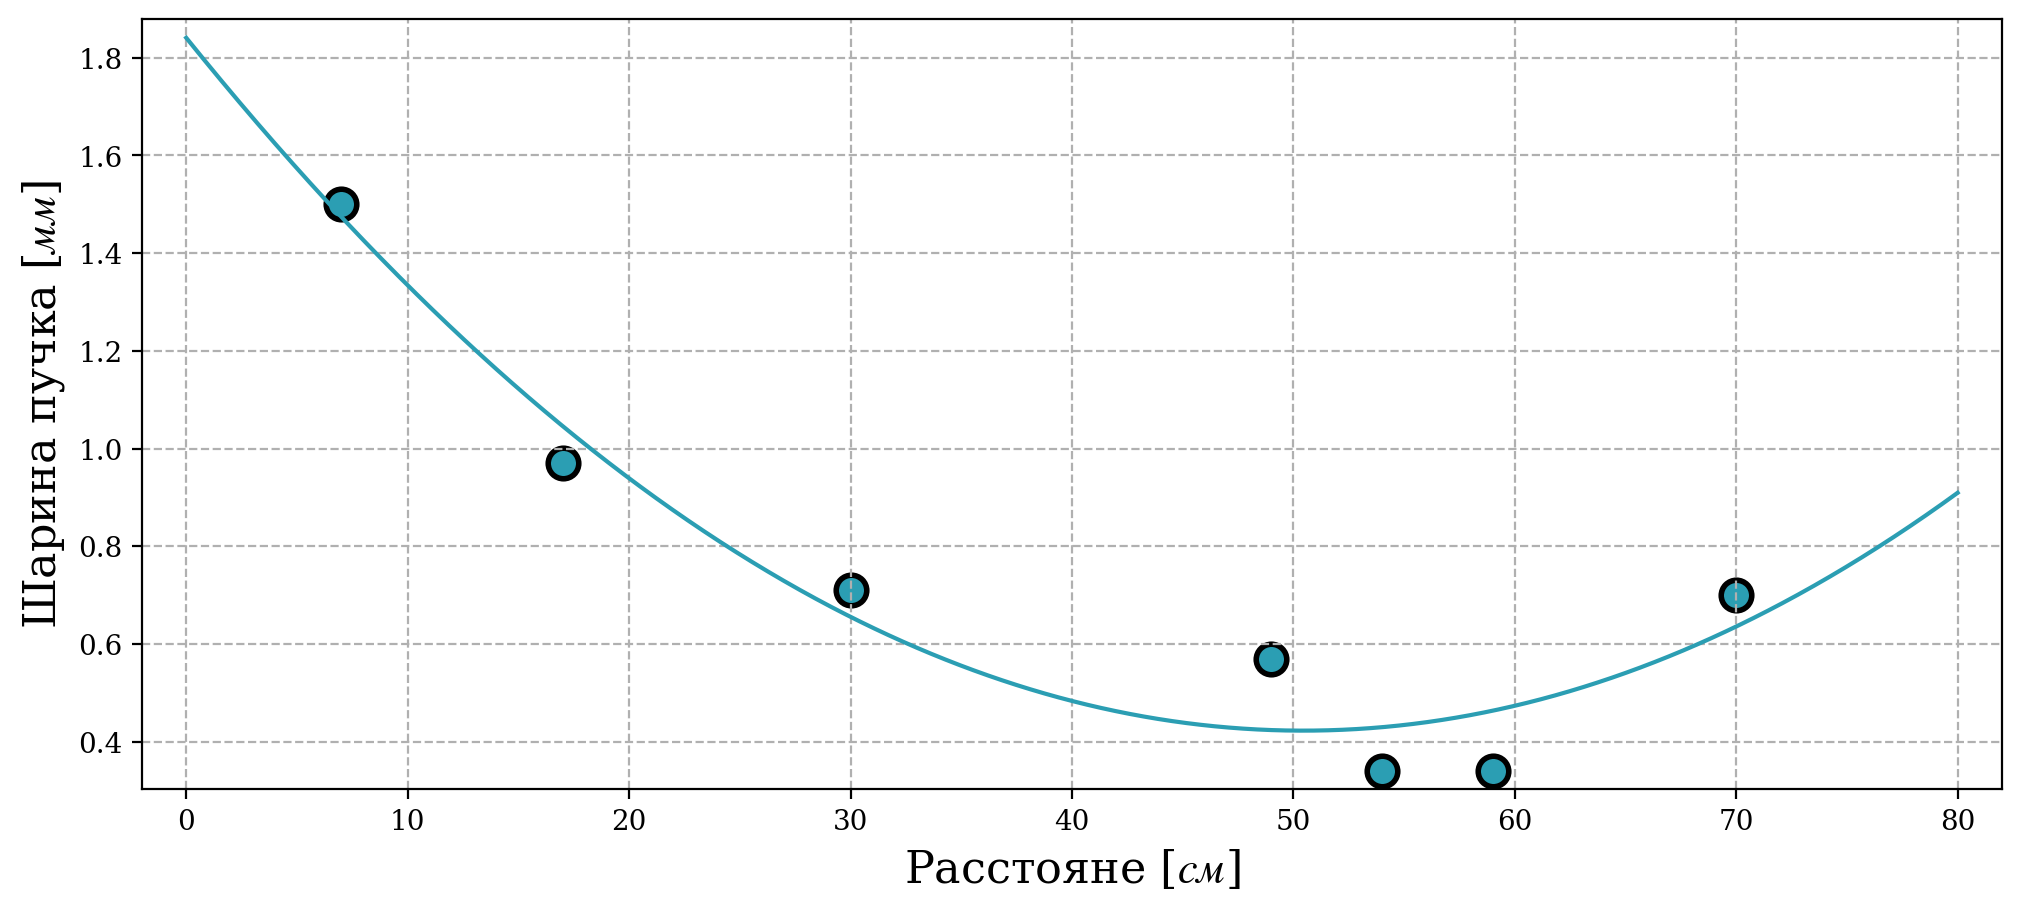
\includegraphics[width = 0.95\textwidth]{red.png}
    \caption{Зависимость ширины пучка от расстояния до лазера}
    \label{fig:1}
\end{figure}

Аналогично снимем зависимость ширины пучка от расстояния между фотодиодом и полупроводниковым  лазером. 
Полученная зависимость гораздо хуже приближается параболой. Это может быть связано с тем, что по мере удаления фотоприемника от лазера, излучение переставало попадать на щель. Тем не менее, оценочно, координата перетяжки:
$x \sim 60$ см (смотрите рисунок 3).

\begin{figure}[htbp]
    \centering
    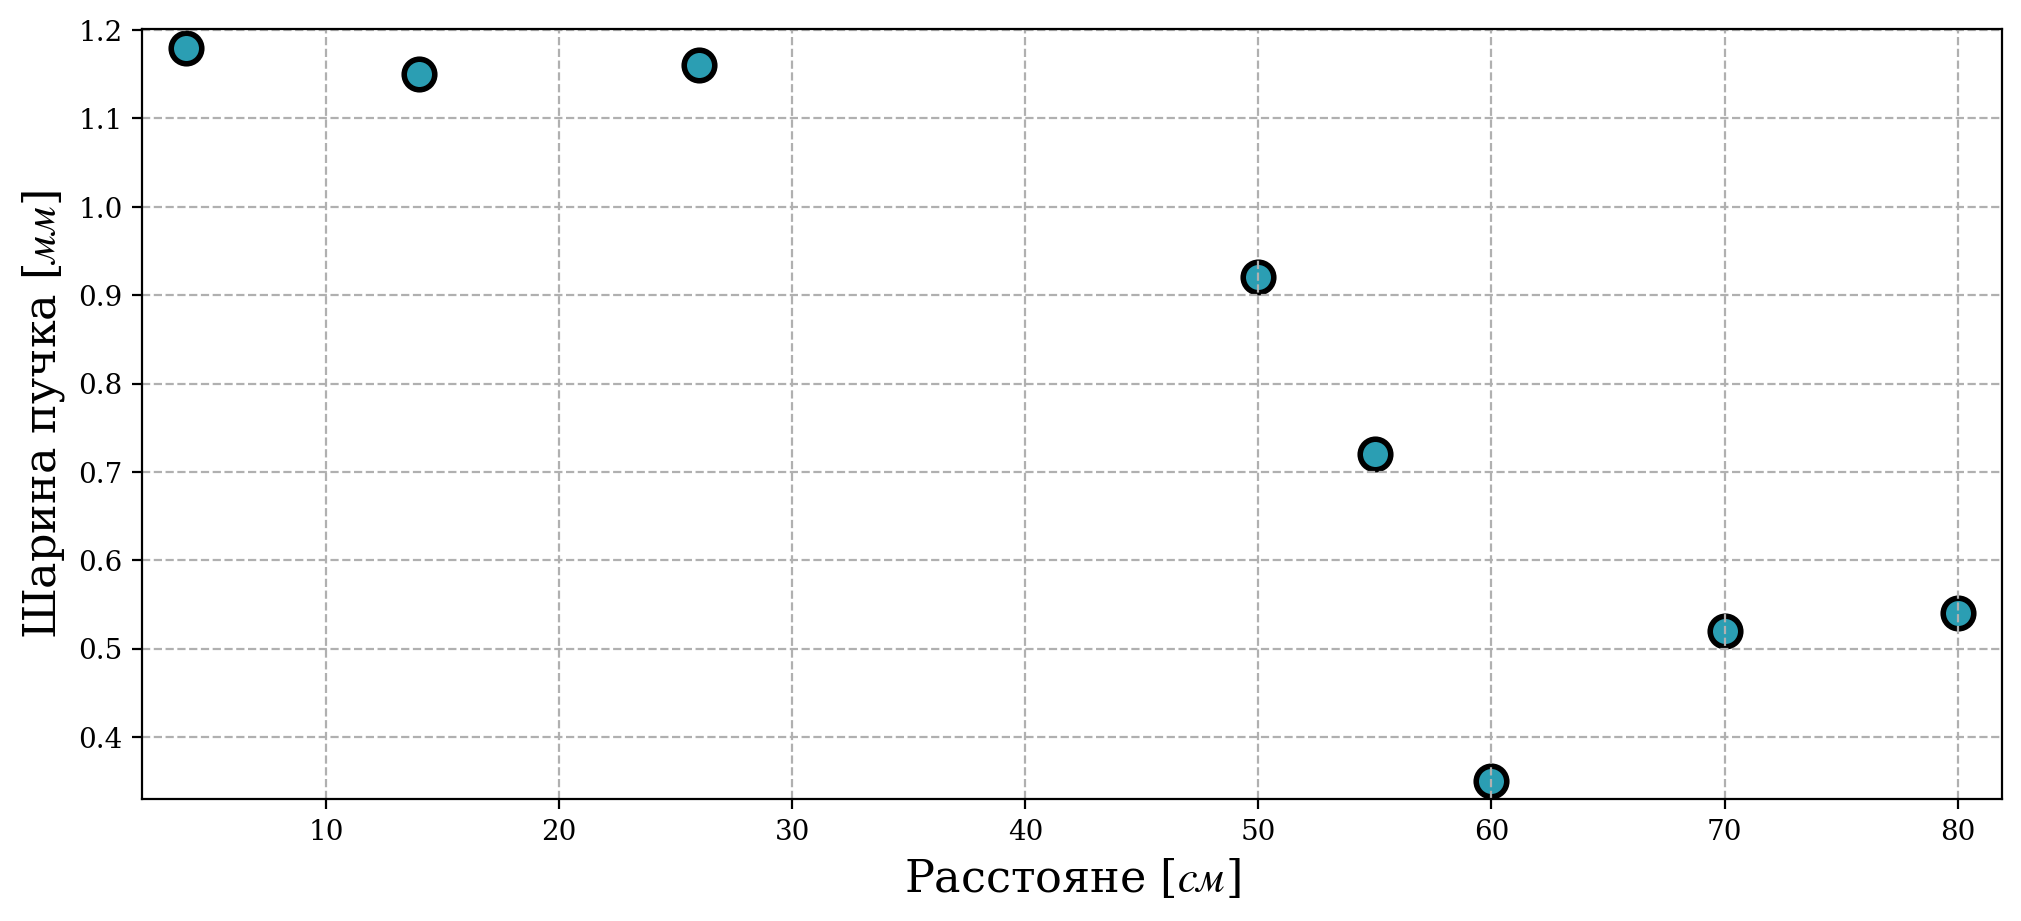
\includegraphics[width = 0.95\textwidth]{green.png}
    \caption{Зависимость ширины пучка от расстояния до полупроводникового лазера}
    \label{fig:2}
\end{figure}


\section*{\textcolor{header}{Вывод}}

В данной работе было исследовано распределение интенсивности излучения лазеров в зависимости от расстояния между лазером и щелью фотоприемника. В частности, по измеренной ширине пучка от расстояния была оценочно получена координата перетяжки.




\end{document}
